\section{Koncepcja mapowania obiektów na format CSV}

Opracowana została struktura pliku .csv, umożliwiająca efektywne mapowanie obiektów, do tego formatu. Pozwala ona na zapis wartości prymitywnych, list takich wartości, obiektów oraz list obiektów. Każdy zapisany obiekt, otrzymuje losowy identyfikator \mintinline{php}|uniqueid()|\footnote{https://www.php.net/manual/en/function.uniqid.php}, natomiast obiekty różnych klas zapisywane są w różnych plikach. Nazwy tych plików odpowiadają przestrzenią nazw tych klas w PHP. \\ \newline
W pierwszej linijce pliku .csv - nagłówku, przechowujemy informacje opisujące dane, są to, między innymi: nazwy pól w mappowanej klasie, wartości prefiksowane przy pomocy znaku "\textbf{\~}" informują nas o listach, natomiast wartości zawierające znak "\textbf{@}" wskazują na referencje do  obiektów (np. obiektów innej klasy). Dodatkowemu polu \textbf{id}, przypisano znak specjalny: "\textbf{\#}", tak aby nie kolidował z rzeczywistym polem \textit{id}, które często jest używane w obiektach. Znaki te zostały wybrane, ze względu na brak możliwości wystąpienia ich w rzeczywistej nazwie pola w języku PHP. Pozostała zawartość pliku csv nazywana przez nas \textit{ciałem}, zawiera rzeczywiste mapowanie do obiektów, opisane według definicji z nagłówka.

\paragraph{Przykład mappowania:} Klasa Student i Ocena 



\begin{figure}[ht]
	\centering
	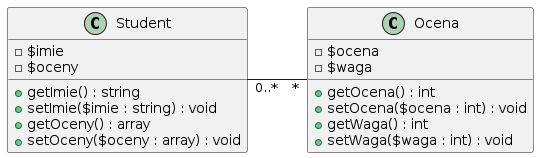
\includegraphics[width=0.8\textwidth]{materiały/st-oc}
	\caption{Mapowane klasy}
\end{figure}


\begin{empty}
	\begin{minted}[
		startinline,
		linenos,
		frame=lines,
		framesep=2mm,
		baselinestretch=1.2,
		fontsize=\footnotesize,
		breaklines,
		obeytabs=true,
		tabsize=2,
		]{text}
imie; ~oceny@TestListsObjs\Ocena; id#
Adam; 6664a3116c12c,6664a3116c131, ... ,6664a3116c13d; 6664a3116c124
	\end{minted}
	\vspace{-10pt}
	\captionof{listing}{Plik TestListsObjs-Student.csv}
\end{empty}
\vspace{10pt}
\begin{empty}
	\begin{minted}[
		startinline,
		linenos,
		frame=lines,
		framesep=2mm,
		baselinestretch=1.2,
		fontsize=\footnotesize,
		breaklines,
		obeytabs=true,
		tabsize=2,
		]{text}
ocena; waga; id#
6; 1; 6664a3116c12c
5; 2; 6664a3116c131
...
1; 6; 6664a3116c13d
	\end{minted}
	\vspace{-10pt}
	\captionof{listing}{Plik TestListsObjs-Ocena.csv}
\end{empty}

\section{Wykorzystanie}
Jak zostało wspomniane we wstępie, aby użyć mappera należy, wykorzystywać trait \mintinline{php}|CSVMapperInjector| oraz wywoływać pozyskaną metodę \mintinline{php}|injectDependencies()|.

\begin{empty}
	\begin{minted}[
		startinline,
		linenos,
		frame=lines,
		framesep=2mm,
		baselinestretch=1.2,
		fontsize=\footnotesize,
		breaklines,
		obeytabs=true,
		tabsize=2,
		]{php}
<?php
	require 'fake_vendor/autoload.php';
	require 'vendor/autoload.php';
	use CSVMapper\Boostrapper\CSVMapperInjector;
	
	class App 
	{
		use CSVMapperInjector;
		
		public function __construct ()
		{
			$this->injectDependencies();
		}
		
		/**
		* @CSVMapper
		*/
		private $csvMapper;
		
		public function main ()
		{
			var_dump($this->csvMapper);
		}
		
	}
	
	(new App())->main();
	\end{minted}
	\vspace{-10pt}
	\captionof{listing}{Przykład powołania mappera.}
\end{empty}

Mając już obiekt, \mintinline{php}|csvMappera|, możemy dokonywać operacji mapowania obiektów z pliku, jak i również ich zapisywania. Przy pomocy metod \mintinline{php}|read()| oraz \mintinline{php}|save()|.

\begin{empty}
	\begin{minted}[
		startinline,
		linenos,
		frame=lines,
		framesep=2mm,
		baselinestretch=1.2,
		fontsize=\footnotesize,
		breaklines,
		obeytabs=true,
		tabsize=2,
		]{php}
public function main ()
{
	$myClass = new MyClass();
	$this->csvMapper->save($myClass);
}
	\end{minted}
	\vspace{-10pt}
	\captionof{listing}{Przykład zapisu obiektu klasy \textbf{MyClass} do pliku.}
\end{empty}


\begin{empty}
	\begin{minted}[
		startinline,
		linenos,
		frame=lines,
		framesep=2mm,
		baselinestretch=1.2,
		fontsize=\footnotesize,
		breaklines,
		obeytabs=true,
		tabsize=2,
		]{php}
public function main ()
{
	$myObject = $this
		->csvMapper
		->read("./MyClass.csv", MyClass::class);
	
	var_dump($myObject);
}
	\end{minted}
	\vspace{-10pt}
	\captionof{listing}{Przykład odczytu obiektu klasy \textbf{MyClass} z pliku.}
\end{empty}